% !TEX options=--shell-escape
\documentclass [12pt]{article} 

\usepackage {amsmath}
\usepackage {amsthm}
\usepackage {amssymb}
\usepackage {graphicx} 
\usepackage {float}
\usepackage {multirow}
\usepackage {xcolor}
\usepackage {algorithmic}
\usepackage [ruled,vlined,commentsnumbered,titlenotnumbered]{algorithm2e} \usepackage {array} 
\usepackage {booktabs} 
\usepackage {url} 
\usepackage {parskip} 
\usepackage [margin=1in]{geometry} 
\usepackage [T1]{fontenc} 
\usepackage {cmbright} 
\usepackage [many]{tcolorbox} 
\usepackage [colorlinks = true,
            linkcolor = blue,
            urlcolor  = blue,
            citecolor = blue,
            anchorcolor = blue]{hyperref} 
\usepackage {enumitem} 
\usepackage {xparse} 
\usepackage {verbatim}
\usepackage{listings}
\usepackage{xcolor}
\usepackage[cache=false]{minted}
\usepackage{mdframed}

\BeforeBeginEnvironment{minted}{\begin{mdframed}}
\AfterEndEnvironment{minted}{\end{mdframed}}

\DeclareTColorBox {Solution}{}{breakable, title={Solution}}
\DeclareTColorBox {Solution*}{}{breakable, title={Solution (provided)}}
\DeclareTColorBox {Instruction}{}{boxrule=0pt, boxsep=0pt, left=0.5em, right=0.5em, top=0.5em, bottom=0.5em, arc=0pt, toprule=1pt, bottomrule=1pt}
\DeclareDocumentCommand {\Expecting }{+m}{\textbf {[We are expecting:} #1\textbf {]}}
\DeclareDocumentCommand {\Points }{m}{\textbf {(#1 pt.)}} 

\begin {document} 

{\LARGE \textbf {COMP 285 (NC A\&T, Spr `22)}\hfill \textbf {Homework 1} } 
\vspace {1em} 
\begin {Instruction} 

\paragraph {Due.} Tuesday, January 25th, 2022 @ 11:59 PM!
\end {Instruction} 

\vspace {1em} 
\begin {Instruction} \paragraph {Homework Expectations:} Please see the \href{https://www.comp285.ml/homework/#general-homework-information}{Homework} part of the Course Website (\href{https://www.comp285.ml/policies/#collaboration-policy-and-honor-code}{comp285.ml/policies}) for guidance on what we are looking for in homework solutions. We will grade according to these standards, and you should cite all sources you used outside course material.

\paragraph {What we expect:} Make sure to look at the ``\textbf {We are expecting}'' blocks below each problem to see what we will be grading for in each problem! \end {Instruction}

\vspace {1em} 
\begin {Instruction} 

\paragraph {Exercises} The following questions are exercises. We suggest you do these on your own. As with any homework question, though, you may ask the course staff for help.

\paragraph {Points} This assignment is worth a total of 100 points.
\end {Instruction} 

\begin{centering}
\section*{Fun with Algorithms}
\end{centering}

This course will be a mixture of written homework and coding assignments. Both types of assignments will be submitted through \href{https://www.gradescope.com/courses/350304}{Gradescope}.

In order to reduce the overhead to the course staff, all coding assignments will be released through \href{https://repl.it/}{repl.it}, an in-browser IDE. \textit{This will be the only supported IDE} for the class.

By \textit{supported}, we mean that if you run into issues on \href{https://repl.it/}{repl.it}, the course staff will do everything in their power to resolve them. We \textit{strongly encourage} you to use repl.it for the coding portions of the homework assignments.


\section {Exercise: Setting up repl.it}
\Points{20} As such, the this graded exercise will walk you through setting up your \href{https://repl.it/}{repl.it} account, joining the course, and getting your copy of the starter code. Even if you \textbf{do not plan} to use \href{https://repl.it/}{repl.it} for writing/developing your solutions (because you have another preferred IDE), you will use it to obtain your starter code. 

First, let's start by getting you an account and joining the right project:

\begin{enumerate}
    \item If you don't already have a repl.it account with your ``aggies.ncat.edu'' email, head over to the repl.it \href{https://repl.it/}{homepage}. On the top-right, click the `Sign Up' and use your NCAT email address to sign-up.
    \item Complete the registration process (eg, there's a verification email you should get)
    \item Join the @COMP285 Team by following \href{https://repl.it/teams/join/axywewyfiltmqtcgovikrywbqisfdgss-COMP285}{this link}.
\end{enumerate}

Next, let's get your starter code. From your repl.it homepage, you should have a menu down the left-hand side of the page (if not, maybe click the hamburger menu to open it?). Click on "Teams" as shown in Figure \ref{fig:replit_homepage}. You should see `North Carolina A\&T' under `Education', as well as the `COMP 285' Team Project.

Click on `COMP 285', which will take you to the Team Homepage. From there, under `Projects', you should see a link to get started on HW1-Code. Clicking it will give you the starter code, as well as set you up with an online. 

If the above does not work, you can also try going directly to the \href{https://replit.com/team/COMP285/HW1-Code}{project link}.

\begin{figure}[h!]
\centering
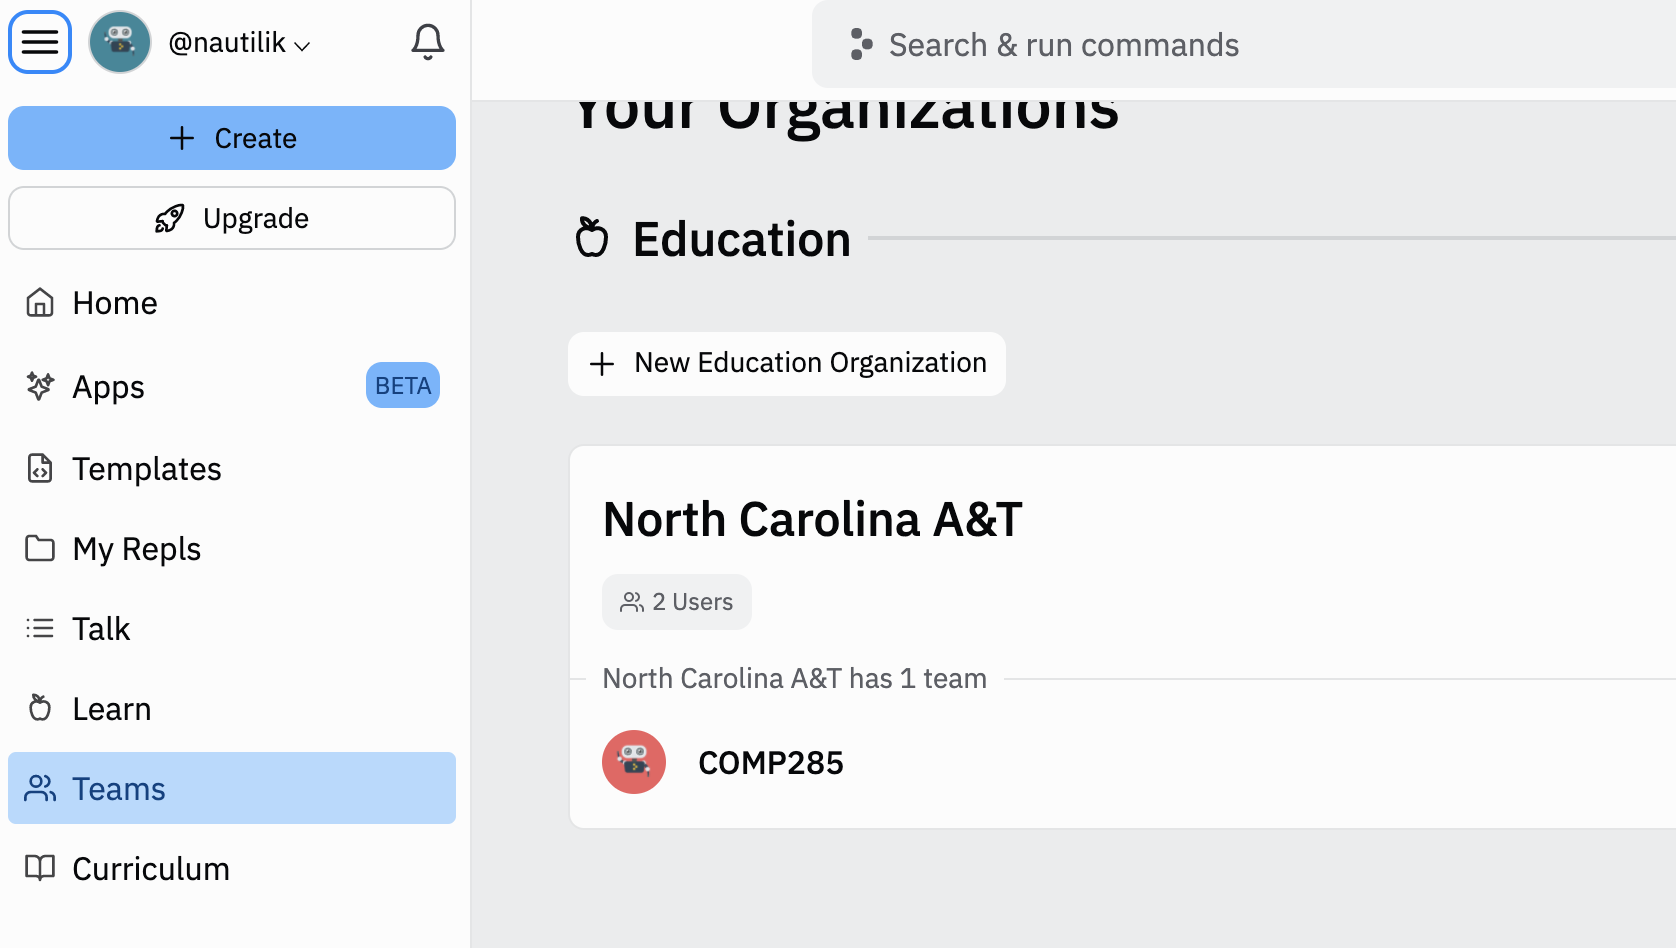
\includegraphics[scale=0.5]{replit.png}
\caption{View of the repl.it Homepage for a student.}
\label{fig:replit_homepage}
\end{figure}

Either way, you should now have the starter code. Clicking the big green button at the top of the IDE will execute the \texttt{main} function defined in \texttt{main.cpp}. It'll fail, but that's okay. The rest of the assignment will walk you through implementing different functions in your starter code.


\Expecting{You should have a copy of your starter code now available! You can use replit to make edits and run your code. The course staff can see who has started the project, so that is how you'll get credit for this question. No need to submit anything}


\pagebreak
\section{Interview Practice: Who's Missing!}

\Points{20} Trinitee is just wrapping up her software engineering internship at Foogle \footnote{This is a meant to be a fake company.}. She recently developed an algorithm, \texttt{genereateIDs}, that gives unique IDs, starting from $0$ and in increasing order, to each Google account in a particular region. This is how she defined her algorithm, in a `.h' file.

\vspace{2em}

\begin{minted}[linenos=true]{cpp}
#include <vector>

// Returns a list of unique IDs for the specified `region'.
//
// `region' is a string that specifies a county, place, or location.
// This algorithm looks up every Foogle account in the location,
// and assigns a unique ID. IDs are generated sequentially
// (starting at with 0) and up to `n-1', where `n' is the number
// of people in the given region.
//
// For example:
//      If a region has 3 accounts, return {2, 0, 1}.
//      If a region has 5 accounts, return {1, 0, 3, 2, 4};
//
// Note that the returned IDs are not necessarily sorted.
std::vector<int> generateIDs(const std::string& region);
\end{minted}

However, she's running into a few issues with her code. It seems that the returned vector is always too small - precisely, it seems to always be \textit{exactly one element} too small. 


For example, Trinitee knows that in the country of Algolandia \footnote{This is a fake country! Don't worry if you've never heard of it!}, there are exactly $2^{20} = 1,048,576$ accounts. However, when she runs the following lines of code:

\vspace{2em}
\begin{minted}[linenos=true]{cpp}
const auto ids = genereateIDs("Algolandia");
std::cout << "Length of my ids: " << ids.size();
\end{minted}

It prints $1,048,575$, which is precisely one short. Confused, Trinitee decides to ask Asha, a fellow intern, for some help.

\subsection{Is it sorted?}
\Points{5} Asha suggest to Trinitee that they first write a program to check if the IDs she's getting back are \textbf{sorted in descending order}. She thinks that if they're sorted, it'll be easy for them to find which one is missing!

She starts writing out the program to do this (check if a vector of integers is \textbf{sorted in descending order}), but suddently, someone comes a long and deletes part of her code! Below is what she has left.

\vspace{2em} 

\begin{minted}[linenos=true]{cpp}
// Checks if a vector<int> called `elements' is sorted in
// descending order. That is:
// {1, 2, 3, 4} returns false, because it's sorted but increasing.
// {4, 3, 2, 1} returns true, because it's sorted and decreasing.
bool isSortedDescending(const std::vector<???>& elements) {
    for (int i = 0; i < element.size(); i++) {
        if (???) {
            return false;
        }
    }
    return true;
}
\end{minted}

Flabergasted, Asha turns to you for help!

\begin{enumerate}
    \item \Points{2} What should go in the first set of `???' in line 5 above? \footnote{If you're having trouble, read the comment for the function carefully!}
    \item \Points{2} What should go in the second set of `???' in line 7 above? \footnote{If you're having rouble, this is very similar to what we did in class, but instead of \textbf{ascending}, here we want to check if the list is \textbf{descending}.}
    \item \Points{1} What is the big-Oh running time of the \texttt{isSortedDescending} function, if we let $n$ be the number of elements?
\end{enumerate}

\Expecting{You should provide an answer for each of the three sub-questions above. The first two are snippets of code (just write it out), and the last one should be $O(\dots)$ where you fill-in the $\dots$. In total, they are worth 5 points out of 20 for this problem.}

\subsection{So what account is missing?}
\Points{5} Sadly, it turns out the lists are not sorted! I guess the documentation was right this time! You, Trinitee, and Asha start brainstorming other solutions. How can we figure out which ID is the one that's missing?

Trinitee gives another suggestion. On the white board, she writes the numbers:
$$
0, 1, 2, 3, 4, 5, 6, 7
$$

And asks:

\begin{enumerate}
    \item [2.2.1] \Points{1} What do the numbers above add up to? 
\end{enumerate}

She then erases the numbers, and writes:
$$
(0, 7); (1, 6); (2, 5); (3, 4)
$$

She turns to you, and asks:

\begin{enumerate}
    \item [2.2.2] \Points{1} What do each of the pairs add up to? How many pairs are there?
\end{enumerate}

After thinking about the above for a bit, all three of you jump up excitedly! Asha goes to the board and writes:
$$
0, 1, 2, 3, 4, \dots, n-3, n-2, n-1, n
$$

and then writes:

$$
(0, n); (1, n-1); (2, n-2); (3, n-3); (4, n-4), \dots
$$

Turns out both Asha and Trinitee are quite smart! They turn to you, and ask:

\begin{enumerate}
    \item [2.2.3] \Points{3} If we add up all the numbers from $0$ to $n$, what do they add up to? Is there a closed-form formula? \footnote{If you're having trouble, check-out this \href{https://www.youtube.com/watch?v=aaFrAFZATKU&t=343s}{video}}
\end{enumerate}

\Expecting{An answer for each of the above questions. The first two should be a number, and the last should be a formula which uses $n$.}


\subsection{Finding The Missing ID}
\Points{10} Having figured out the above, the three of you start coding! You come up with the following pseudo-code:

\begin{verbatim}
algorithm discoverMissingID
  Input: The output from the malfunctioning generateIDs function above.
  Output: The missing ID.

  s1 = the sum of all numbers in the given vec<int>
  s2 = what the sum should be if no numbers were missing. See answer to 2.2.3.
  return s2 - s1
\end{verbatim}

Now, Trinitee and Asha look at you, and say: "Can you code it up for us?"

\Expecting{You should implement the above pseudo-code in \texttt{answers.cpp}, which is part of the starter code you retrieved in Exercise 1}.


\pagebreak
\section{Interview Practice: The Best Basketball Player}
\Points{20} Hassan has been following closely the latest happening with the Denver Nuggest \footnote{If you're like me and do now know who they are, suffice it to say that they're a basketball team}. He's a bit disappointed with their performance this season, so he reaches out to his friend Caleb. 

Caleb is a data scientist working for the U.S. Census. He tells Hassan that a big issue with the Denver Nuggest this season is that they're players are too short! What they really need is a tall player - wait, not a tall player, \textbf{the tallest player} in America.

Thankfully, Caleb has just the data for the job! He shows Hassan that the census collects every person's height as an integer in inches \footnote{This is not true. It would be a violation of privacy if it was...} (they're too lazy, so they always round to the nearest inch).


\subsection{Finding the Tallest American}
\Points{10} Hassan and Caleb feel like they've done a good job so far, so they reach out to you. They know you're an expert in C++, do they ask you to write a function - \texttt{findTallestPerson} - which takes in a vector of integers correspondong to each person's height from the census data Caleb has, and returns \textbf{the index} of the largest height. If there are multiple largest heights, it returns the smaller index.

They give you the following examples:

\vspace{2em}
\begin{minted}[linenos=true]{cpp}
findTallestPerson({1, 3, 4, 5, 2});  // should return 3, the index of 5
findTallestPerson({-1, -3, -4, -5, -2});  // should return 0, the index of -1
findTallestPerson({});  // should throw std::invalid_argument
\end{minted}

You look at them a bit funny, and wonder to yourself: "Who in the world has negative height? And why would the list ever be empty?" Still, you want to do a good job, so you do what they ask.

\Expecting{You should implement \texttt{findTallestPerson} in \texttt{answers.cpp}, which is part of the starter code you retrieved in Exercise 1}.


\subsection{Is it Correct?}
\Points{5} After implementing the above algorithm, you want to show all your friends how good you've gotten at \textit{correcness} and \textit{runtime} analysis. You write down the pseudocode:

\begin{verbatim}
algorithm findTallestPerson
    Input: A vector of integers representing height in inches
    Output: The index of the tallest person.

    if input is empty:
        throw error

    tallestIndex = 0
    for index in {1, ..., input.size() - 1}:
        if input[index] > input[tallestIndex]:
            tallestIndex = index
    return tallestIndex
\end{verbatim}

You want to \textit{prove} to Caleb and Hassan the algorithm above is correct. You start walking them through a proof by induction. Fill out the missing pieces.

\begin{itemize}
    \item \textbf{Inductive Hypothes}: \texttt{tallestIndex} points to the index of the largest element in \texttt{input[:i+1]} after the $i$-th iteration (of the for loop)
    \item \Points{3} \textbf{Base Case (i=0)} \textit{TODO: FILL THIS OUT}
    \item \Points{2} \textbf{Inductive step} Assume our \textbf{inductive hypothesis} is true for $i = k$ (eg, at the $k$-th) iteration. \textit{Explain why} it will also be true for $i = k + 1$ (eg, at the next iteration of the for-loop).
    \item \textbf{Conclusion}: As shown above, the inductive hypothesis holds for $i = 0$, (\textbf{base case}). We also argued as part of the \textbf{inductive step}, that if it holds for $i=0$, it is also true for $i=1$, and if it's true for $i =1$, it's true for $i=2$, and so on. As such, it must be true for $i = n -1$ (aka, when our for-loop finishes). Therefore, \texttt{tallestIndex} points to the index of the largest element in \texttt{input[:n]} after the $n-1$-th iteration, which is exactly what we wanted.
\end{itemize}


\Expecting{You should provide written responses to the two missing pieces in the above proof. The first is the base case, the second is an explanation for why the inductive step works.}

\subsection{How fast is it?}
\Points{5} You also want to show everyone how good you are at analyzing the runtime of your algorithm. For your reference, you write down the formal definition of big-Oh: $T(n)= O(g(n))$ if and only if:
$$
\exists c, n_0 \text{ s.t. } \forall n > n_0, T(n) \leq c \cdot g(n)
$$

Then, you answer the following:
\begin{itemize}
    \item \Points{2} What is the big-Oh runtime of the pseudo-code shown above?
    \item \Points{2} After practicing the guitar, Vincent (another amazing C++ coder),  tells you: ``I implemented your code, and counted up all the operations. There are exactly $T(n) = 3n + 1$ operations in my implementation! I think $T(n) = O(n)$''. What values of $c, n_0$ would convince you that Vincent is right, and his implementation is in-fact $O(n)$?
    \item \Points{1} Vincent thinks for a bit, and says - I think $T(n) = O(n^2)$! Is he right? If yes, what are the $n_0$ and $c$ values that convince you he's right? If no, briefly explain why such values cannot exist.
\end{itemize}

\Expecting{And answer to each of the above. The first should be of the form $O(\dots)$, where you've filled in the $\dots$. The second should be two numbers, the $c$ and $n_0$ that convince you. The last should be either two numbere (the $c$ and $n_0$ that convince you), or a short sentence explaning why they don't exist.}



\pagebreak
\section{Interview Practice: Game Development}
\Points{20} Nkumbu is a world-renowed game developer working for Big Corp Studios \footnote{Again, fake name.}. His game works by randomly generating pets, each which costs a random amount of coins (only integer values). The player is then allowed to purchase precisely \textit{two} pets. 

Being an awesome developer, Nkumbu wants to make sure that no matter how many coins the player has, there are always \textit{two} pets that we can purchase at the cost of all his coins.


\subsection{Finding the Most Expensive Pets}
\Points{10} Having been stumped with this problem for quite a bit, he reaches out to Isaiah, whose an avid gamer and recently took COMP 285: Analysis of Algorithms for help. He asks Isaiah to write a C++ function \texttt{findTwoPets}, which takes as input a vector of integers (corresponding to the cost of each pet) as well as a target value (corresponding to how many coins the player currently has), and returns a pair that represents two \textbf{distinct}\footnote{Should be pretty obvious that we're not going to let a player buy the same pet twice!} indices of pet costs that sum up to the target value.

For some reason, Nkumbu also wants the smaller index to be first. To be super clear, he gives a few examples to Isaiah:

\vspace{2em}
\begin{minted}[linenos=true]{cpp}
std::vector<int> pet_costs = {0, 2, 3, 4, 5};
std::pair<int, int> out1 = findTwoPets(pet_costs, /*coins=*/6);
std::pair<int, int> out2 = findTwoPets(pet_costs, /*coinst*/10);

std::cout << out1.first << " " << out1.second;  // should output 1 3
std::cout << out2.first << " " << out2.second;  // should output -1 -1
\end{minted}

In the first example, \texttt{vec[1] + vec[3] = 2 + 4 = 6}. In the second example, we returned \texttt{-1, -1} because there are not two distinct elements within the vector that sum to 10 (you can't use 5 twice).

Help Isaiah by writing an algorithm (in C++) that solves this problem. Your solution should be written in \texttt{answer.cpp} which is part of the starter code. 

For context, there's a straight-forward $O(n^2)$ algorithm that you can start with (this is probably the first one you'll think of). There is also an $O(n \log n)$ algorithm (Hint: what if the list was sorted?), and even a far more efficient $O(n)$ algorithm.

For this homework, \textit{there are no explicit time complexity constraints} here (i.e. algorithm just needs to work as intended). You \textit{might} receive bonus points if you implement one of the faster ones, though. 

\Expecting{You should implement \texttt{findTwoPets} in \texttt{answer.cpp} which is part of the starter code. It does not need to be the best algorithm, it just needs to work.}

\subsection{Correctness of Algorithm}
\Points{5} For whichever algorithm you implemented, please provide a few sentences \textit{explaning why} it is correct. This does not need to be formal (but feel free to try a proof by induction). 

\Expecting{A few sentences explaining why the algorithm you write works. You can be informal about it, but try to be precise.}

\subsection{Runtime of Algorithm}
\Points{5} For whichiever algorithm you implemented, what is the big-Oh runtime?

\Expecting{An answer in the form of $O(\dots)$ with $\dots$ filled in.}

\pagebreak
\section{Exercise: Refresher on Nodes, Pointers, etc.}
\Points{20} In this exercise, we'll write some code that will set you up for implementing Karatsuba's algorithm later in the class (maybe as extra credit!). 

\subsection{Adding Two Numbers}
\Points{10}
Almost every programming languages already has `+' and `*' implemented for you, on integers. So to make this more interesting, your task is to write the function \texttt{add}, which given two numbers represented as linked lists of single-digit
integers, returns their sum as a linked list of integers. Return the head node.

The linked list is represented as follows:
\begin{minted}[linenos=true]{cpp}
template <typename T>
struct Node {
  T value_;
  Node<T>* next_ = nullptr;
};
\end{minted}

We have provided a util function \texttt{makeList} to convert an integer to its corresponding list representation. Feel free to take a look at the function in \texttt{util.cpp} from the starter code and note how we extract the digits (\texttt{num \% 10} and \texttt{num / 10} in the loop).

For convenience, the list stores the digits from the lowest to the highest, e.g., \texttt{makeList(123) => head -> [3 -> 2 -> 1]}.

Some examples for \texttt{add}:
\begin{minted}[linenos=true]{cpp}
Node<int>* q4bInput1 = makeList(123);  // [3 -> 2 -> 1] 
Node<int>* q4bInput2 = makeList(242);  // [2 -> 4 -> 2]
Node<int>* q4bOut1 = add(q4bInput1, q4bInput2);
std::cout << listToString(q4bOut1)
        << std::endl;  // should output [5 -> 6 -> 3] (meaning 365)
freeList(q4bInput1);
freeList(q4bInput2);
freeList(q4bOut1);

Node<int>* q4bInput3 = makeList(999);
Node<int>* q4bInput4 = makeList(1);
Node<int>* q4bOut2 = add(q4bInput3, q4bInput4);
std::cout << listToString(q4bOut2)
        << std::endl;  // should output [0 -> 0 -> 0 -> 1] (meaning 1000)
freeList(q4bInput3);
freeList(q4bInput4);
freeList(q4bOut2);
\end{minted}

Refresher on pointers, memory allocation, and deallocation for your reference:

\begin{itemize}
    \item To create a \texttt{Node} object, use \texttt{Node<int>* ptr = new Node<int>()}. \texttt{new} dynamically allocates memory for this.
    \item We provided a \texttt{freeList} function that will traverse the linked list and free every node. \texttt{freeList} is all we need here, but always remember when you have allocated memory (i.e. with `new`) to free it when finished (i.e. `delete ptr`).
    \item To check whether there are "memory leaks" (i.e., allocated memory but not deallocated), you can run valgrind on repl.it with `valgrind --leak-check-full ./main`
\end{itemize}

Please note that this question is at the upper-end of the C++ intricacies we will learn on in the course. Having familiarity with pointers here will serve us well later on (e.g. with trees).

\Expecting{You should implement \texttt{add} in \texttt{answers.cpp} in your starter code.}

\subsection{Runtime of Addition}
\Points{10} The algorithm above forces you to implement addition the way you would normally do it by hand (eg, add numbers and carry when they add to more than 10). In this context, let us define ``operation'' as being a 1-digit addition. What is the big-Oh running time of this algorithm, in terms of $n$ where $n$ is the length of the input lists (eg, numbers).

\Expecting{A single answer in the form $O(\dots)$ where you've filled in $\dots$. No need to prove or argue this is correct, simply provide your answer.}


\pagebreak
\section*{Submitting the Assignment}

This assignment is a combination of written and programming questions. Both portions of the assignment should be submitted through \href{https://www.gradescope.com/courses/350304}{Gradescope} before the assignment due date on January 25th, 2022 @ 11:59PM. 

The "Homework 1: Fun with Algorithms" assignment is the written portion, for which you should submit a \textbf{typed} response to the non-coding questions above. Each response should clearly be marked with its corresponding number (for example, 2.1 or 2.2.2) etc. You are free to use the provided templates, or to simply type your responses on a blank document (whatever works for you).

The "Homework 1: Coding" is the programming portion of the assignment. For this portion, download the ".zip" file from replit (see Figure \ref{fig:replit_download}), and upload this ".zip" file as your answer to \href{https://www.gradescope.com/courses/350304}{Gradescope} (see Figure \ref{fig:replit_download}). You can upload the assignment as many times as you want - each time a set of automatic tests will run that test your code for correctness. Feel free to use this to detect when your code is wrong.

\begin{figure}[h!]
\centering
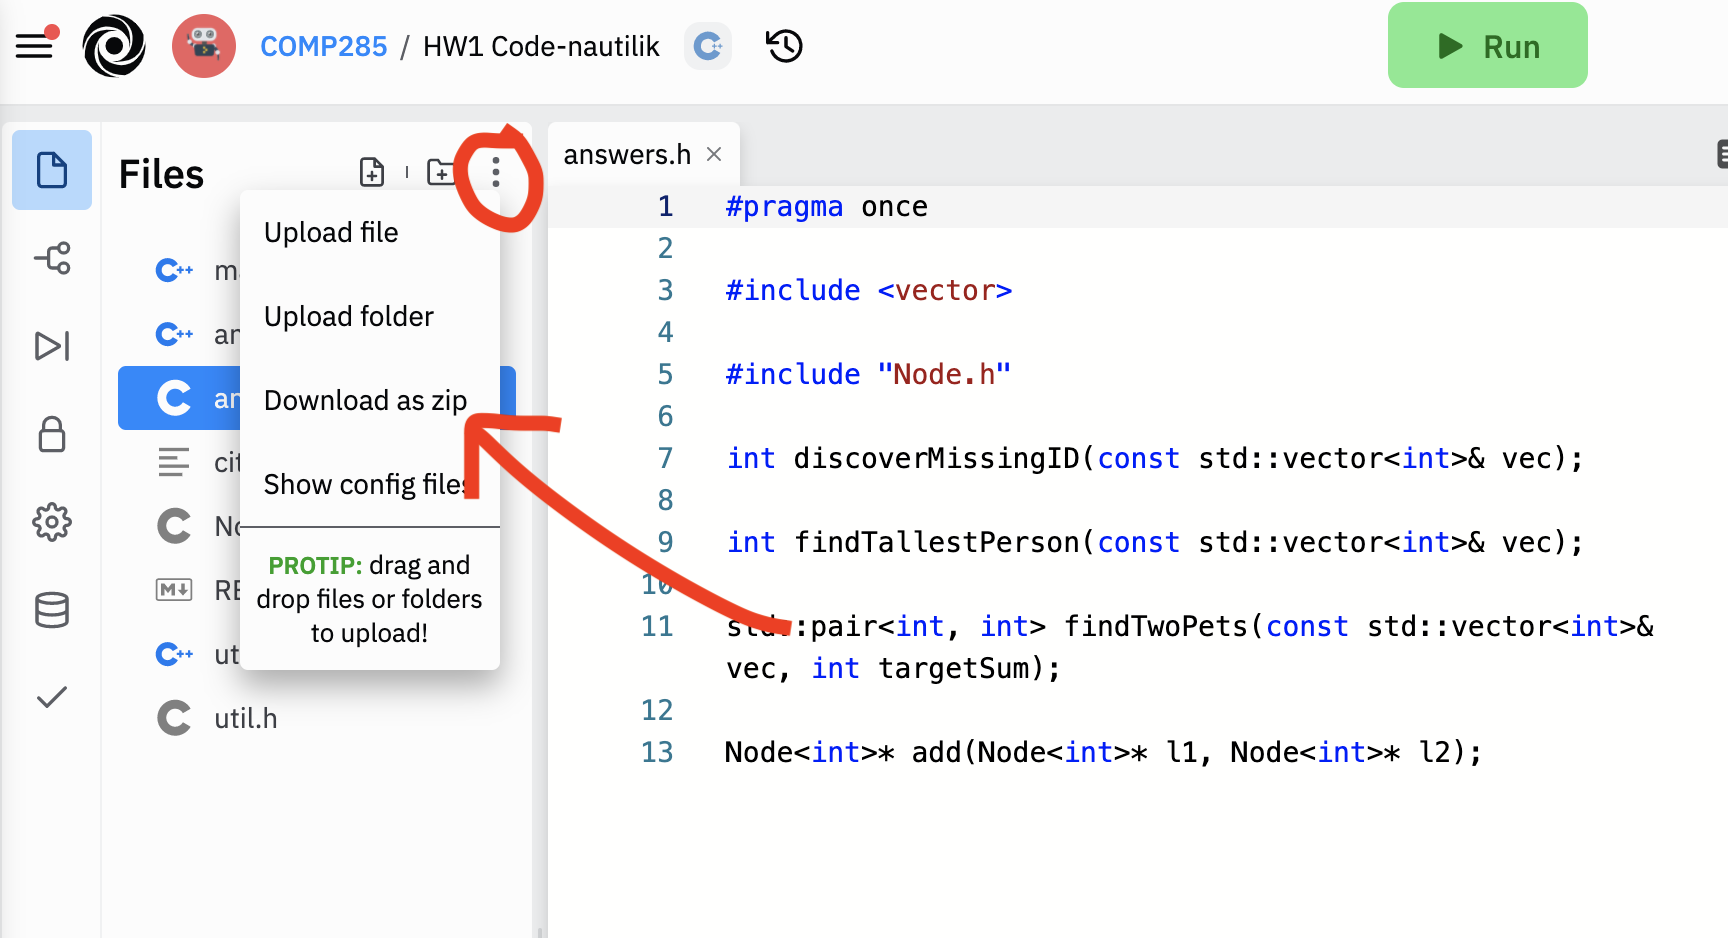
\includegraphics[scale=0.3]{replit-download.png}
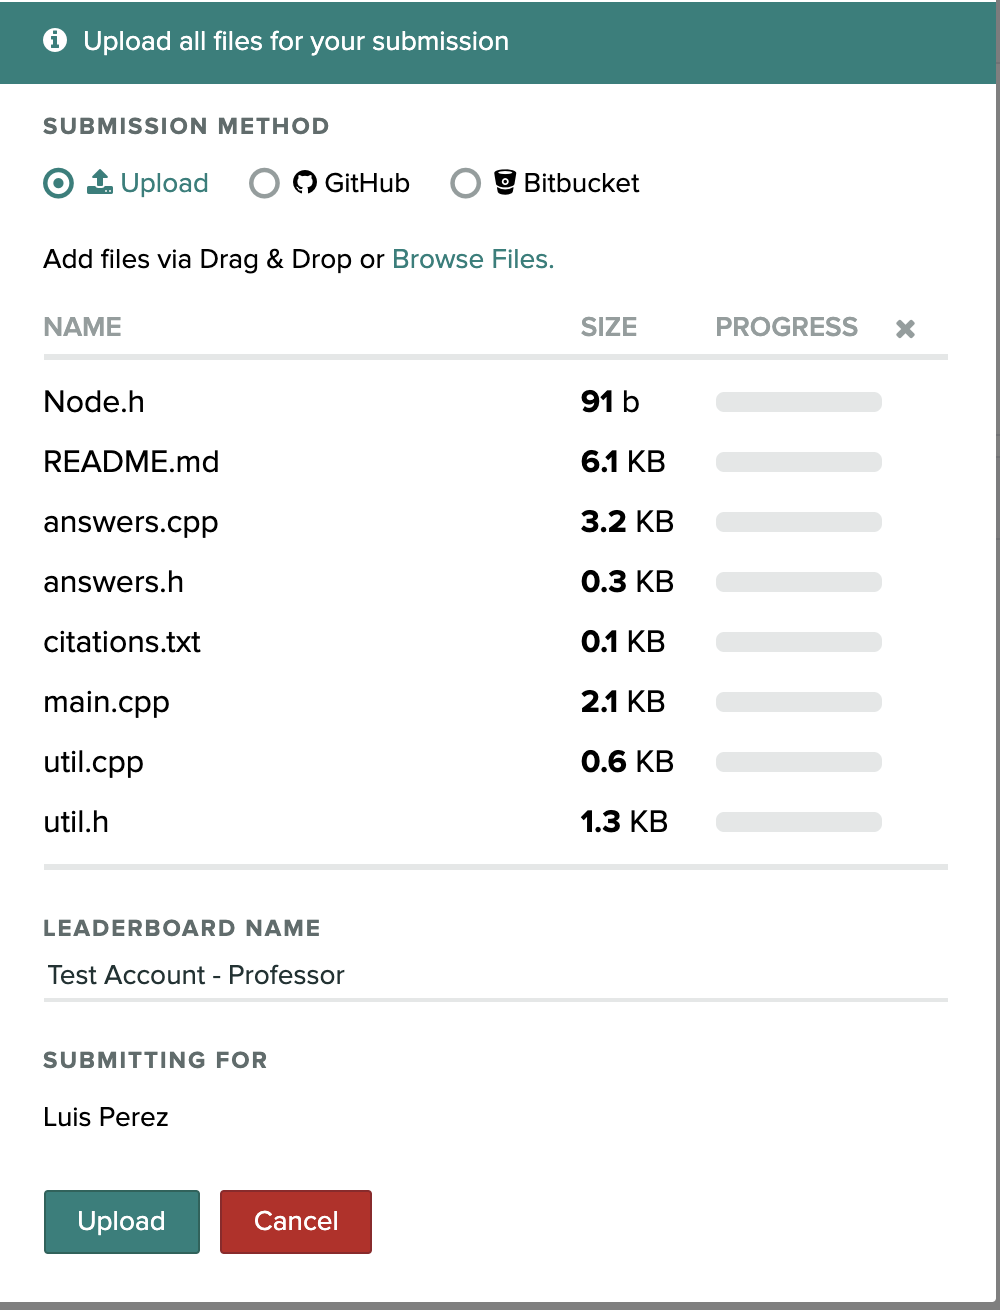
\includegraphics[scale=0.3]{gradescope-upload.png}
\caption{(left) View of the hamburger menu which holds the option to download your source code as a ".zip" which can be directly uploaded to \href{https://www.gradescope.com/courses/350304}{Gradescope}. (right) View of the screen you should see after uploading your ".zip" file. Make sure all the files are present, since they're requires for the autograder to run.}
\label{fig:replit_download}
\end{figure}


To summarize, do the following:
\begin{enumerate}
    \item Submit your \textbf{typed} responses to the non-coding portion of the assignment on Gradescope for "Homework 1: Fun with Algorithms"
    \item Submit your \textbf{code files} as a ".zip" to Gradescope for "Homework 1: Coding".
    \item Fill out this \textbf{Google Form} (\href{https://forms.gle/pvoM4pYV2u4yYXc96}{https://forms.gle/pvoM4pYV2u4yYXc96}) to help me track your thoughts on the homework.
\end{enumerate}


\end {document} 